\documentclass[../masters.tex]{subfiles}

\begin{document}
\graphicspath{{./imgs/}{../imgs/}} %look for images

\section{Linear Models}
In this section we consider probabilistic graphical models of the form shown in Figure \ref{fig_linmod}. Firstly we investigate a model where the states ($X$) and observations ($Y$) are discrete. Models of this form are classically called Hidden Markov Models (HMMs). Secondly we generalise the model to include continuous states and observations. Models of this form are called Latent Linear Dynamical Systems (the famous Kalman Filter model falls into this category).
\begin{figure}[H] 
\centering
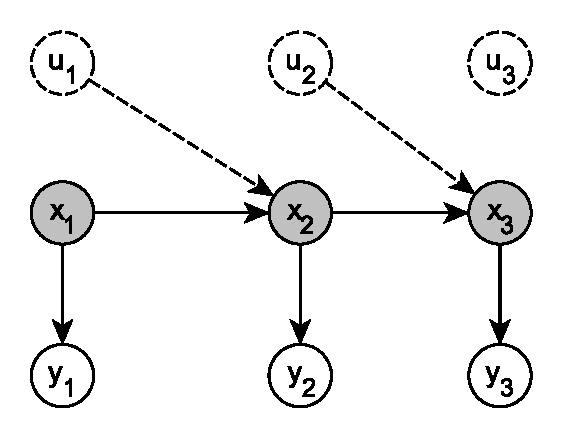
\includegraphics[scale=1.0]{linear_model.pdf}
\caption{Linear Graphical Model}
\label{fig_linmod}
\end{figure}
Intuitively, this model represents the situation where we are not sure about the state of the world but we have some idea represented by the prior $P(X_1)$. At each time step our state changes according to the transition function and we attempt to, amongst other things, infer the new state, perhaps given some observations related to the past and current state.

\subsection{Discrete Models}
In this section we briefly describe Markov Models because they link back to previous work done by the Chemical Engineering Department at the University of Pretoria. We focus on Hidden Markov Models for the remainder of the section because they generalise to Latent Linear Dynamical Systems. 

\subsubsection{Markov Models}
A first order Markov Model (sometimes called a Markov Chain) is shown in Figure \ref{fig_markov_chain}. Using the chain rule for Bayesian Networks we can immediately write down the joint probability distribution as shown in (\ref{eq_markov_chain_joint}).
\begin{equation}
P(X_{1:T}) = \Pi_{t=1}^T P(X_t|X_{t-1}) \text{ with } P(X_1|X_{-1}) = P(X_1)
\label{eq_markov_chain_joint}
\end{equation}  
\begin{figure}[H] 
\centering
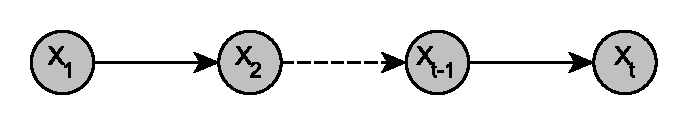
\includegraphics[scale=1.0]{markov_chain.pdf}
\caption{First Order Markov Chain}
\label{fig_markov_chain}
\end{figure}
This model describes the forward propagation of a discrete random variable through time. It is interesting to study the marginal distribution of $P(X_t)$ as it evolves through time. By d-separation we know that $X_t \indep X_{1:t-2} | X_t$. Thus, we only have to marginalise out the previous time step to compute the required distribution as shown in (\ref{eq_markov_chain_marg}).
\begin{equation}
P(X_t) = \sum_{x_{t-1}} P(X_t, x_{t-1}) = \sum_{x_{t-1}} P(x_{t-1})P(X_t|x_{t-1})
\label{eq_markov_chain_marg}
\end{equation}
Since we know that the transition function is a row stochastic $n \times n$ matrix (the random variable has $n$ discrete states) we can write (\ref{eq_markov_chain_marg}) in vector notation (\ref{eq_markov_chain_marg_vec}).
\begin{equation}
P(X_t) = \mathbf{p}_t = \mathbf{A}\mathbf{p}_{t-1} = \mathbf{M}^{t-1}\mathbf{p}_1
\label{eq_markov_chain_marg_vec}
\end{equation}
We have implicitly rewritten (\ref{eq_markov_chain_marg_vec}) in recursive format. Thus we have a recursive expression for the marginal distribution of $X$. If, as $t \rightarrow \infty$, we have that $\mathbf{p}_{t \rightarrow \infty} = \mathbf{p}_{\infty}$ is independent of $\mathbf{p}_1$ we call $\mathbf{p}_{\infty}$ the equilibrium distribution of the chain. 

We define the stationary distribution, in matrix notation, by (\ref{eq_markov_chain_stationary}).
\begin{equation}
\mathbf{p}_{\infty} = \mathbf{A}\mathbf{p}_{\infty}
\label{eq_markov_chain_stationary}
\end{equation}
Recalling the definition of the eigenvalue problem we see that the stationary distribution is just the eigenvector corresponding to the unit eigenvalue of $\mathbf{A}$. While this model may seem simplistic it is the foundation of Google's PageRank algorithm \cite{google}.  Intuitively $\mathbf{p}_\infty$ represents the steady state distribution of the random variable $X$ as it is propagated through time by the transition function $A$.

\subsubsection{Hidden Markov Models}
Hidden Markov Models extend Markov Models by incorporating the observed random variable $Y$ as shown in Figure \ref{fig_linmod}. At each time step it is now possible to observe some value $y_t$ which gives more information about the state of $X_t$. We are still in the setting of discrete random variables. It is not necessary to restrict $Y$ to be discrete but we do so for the sake of simplicity here. In later sections we will model hybrid and purely continuous systems. 

In general a Hidden Markov Model is just a specific case of the general Dynamic Bayesian Network class of graphical models. As such we already know that to fully specify the model we only require a prior state distribution $P(X_1)$, the transition probability function $P(X_t|X_{t-1})$, the observation or emission probability function $P(Y_t|X_t)$ and the Bayesian Network graphs of the initial time step and the next two time steps. We assume that the model's structure repeats at each time step and thus we only require the graph as shown in Figure \ref{fig_linmod}. 

We assume that the transition and observation probability functions are stationary. Consequently they may be represented by the row stochastic square matrices $P(x_t=i|x_{t-1}=j) = \mathbf{A}$ and $P(y_t=i|x_t=j) = \mathbf{B}$. Intuitively this means that the probability of state $x_{t-1}=j$ going to state $x_{t} = i$ is $A_{ij}$. Similarly, $B_{ij}$ is the probability of observing $y_t=i$ if the underlying state is $x_t=j$.

For the purposes of this dissertation we will always assume that the model parameters are known. In the previous section the four primary inference techniques were briefly mentioned. We now derive recursive expressions for each inference technique for discrete models of the form of Figure \ref{fig_linmod}. In the next section we show that these derivations also hold for the continuous case with some minor modifications.

\textbf{Filter:} $P(X_t|y_{1:t})$\\
We start the derivation by noting that $X_{t-1}$ d-separates $X_t$ from $X_{1:t-2}$. Thus $X_{t-1}$ contains all the hidden state information of the system up to and including $t-1$ - this is not surprising since we have assumed a first order Markov system. This is why we consider the reduced state joint $P(X_t, X_{t-1},y_{1:t})$.
\begin{equation}
\begin{aligned}
P(X_t, y_{1:t}) &= \sum_{x_{t-1}} P(X_t, x_{t-1}, v_{1:t-1},v_t)\\
&= \sum_{x_{t-1}} P(y_{1:t-1}, x_{t-1})P(X_t, y_t|y_{1:t}, x_{t-1})\\  & = \sum_{x_{t-1}} P(y_{1:t-1}, x_{t-1})P(X_t|y_{1:t}, x_{t-1})P(y_t|X_t,y_{1:t}, x_{t-1}) \\
&= \sum_{x_{t-1}} P(y_{1:t-1}, x_{t-1})P(X_t|x_{t-1})P(y_t|X_t) \\
\end{aligned}
\label{eq_forward_no_recur}
\end{equation}
Where the expansions followed from the chain rule and the cancellations followed from the conditional independence assumptions of the transition and observation functions. Now we define $\alpha(X_t)=P(X_t,y_{1:t})$. Then (\ref{eq_forward_recur}) follows from (\ref{eq_forward_no_recur}).
\begin{equation}
\begin{aligned}
&\alpha(X_t) = P(y_t|X_t)\sum_{x_{t-1}}P(X_t|X_{t-1})\alpha(X_{t-1}) \text{ for } t>1\\
&\text{with } \alpha(X_1) = P(X_1, y_1) = P(X_1)P(y_1|X_1)
\end{aligned}
\label{eq_forward_recur}
\end{equation}
Clearly we have just derived a recursive expression for the joint distribution $P(X_t, y_{1:t})$. This recursion is called forward recursion in graphical model literature \cite{barber}. To complete our task of estimating $P(X_t|y_{1:t})$ we recall Bayes' Theorem as shown in (\ref{eq_forward_filter}).
\begin{equation}
P(X_t|y_{1:t}) = \frac{P(X_t, y_{1:t})}{P(y_{1:t})} = \frac{\alpha(X_t)}{P(y_{1:t})}
\label{eq_forward_filter}
\end{equation}
Noting that $P(y_{1:t})$ is just a normalisation constant it suffices to normalise $\alpha(X_t)$ to find the filtered distribution of $X_t$ given the observations $y_{1:t})$. One often uses logarithms to perform the filter calculations as machine precision errors become a problem for large $t$ due to the multiplication of small fractions \cite{barber}.

\textbf{Smoothing:} $P(X_t|y_{1:T})$ for $t<T$\\
The smoothing algorithm we study here is called the parallel smoothing algorithm and is often called the Backwards algorithm in literature \cite{murphy1}.


\textbf{Viterbi Decoding:} \\

\textbf{Prediction:} \\


\textbf{Burglar Localisation Problem} \\
xgd
\begin{figure}[H] 
\centering
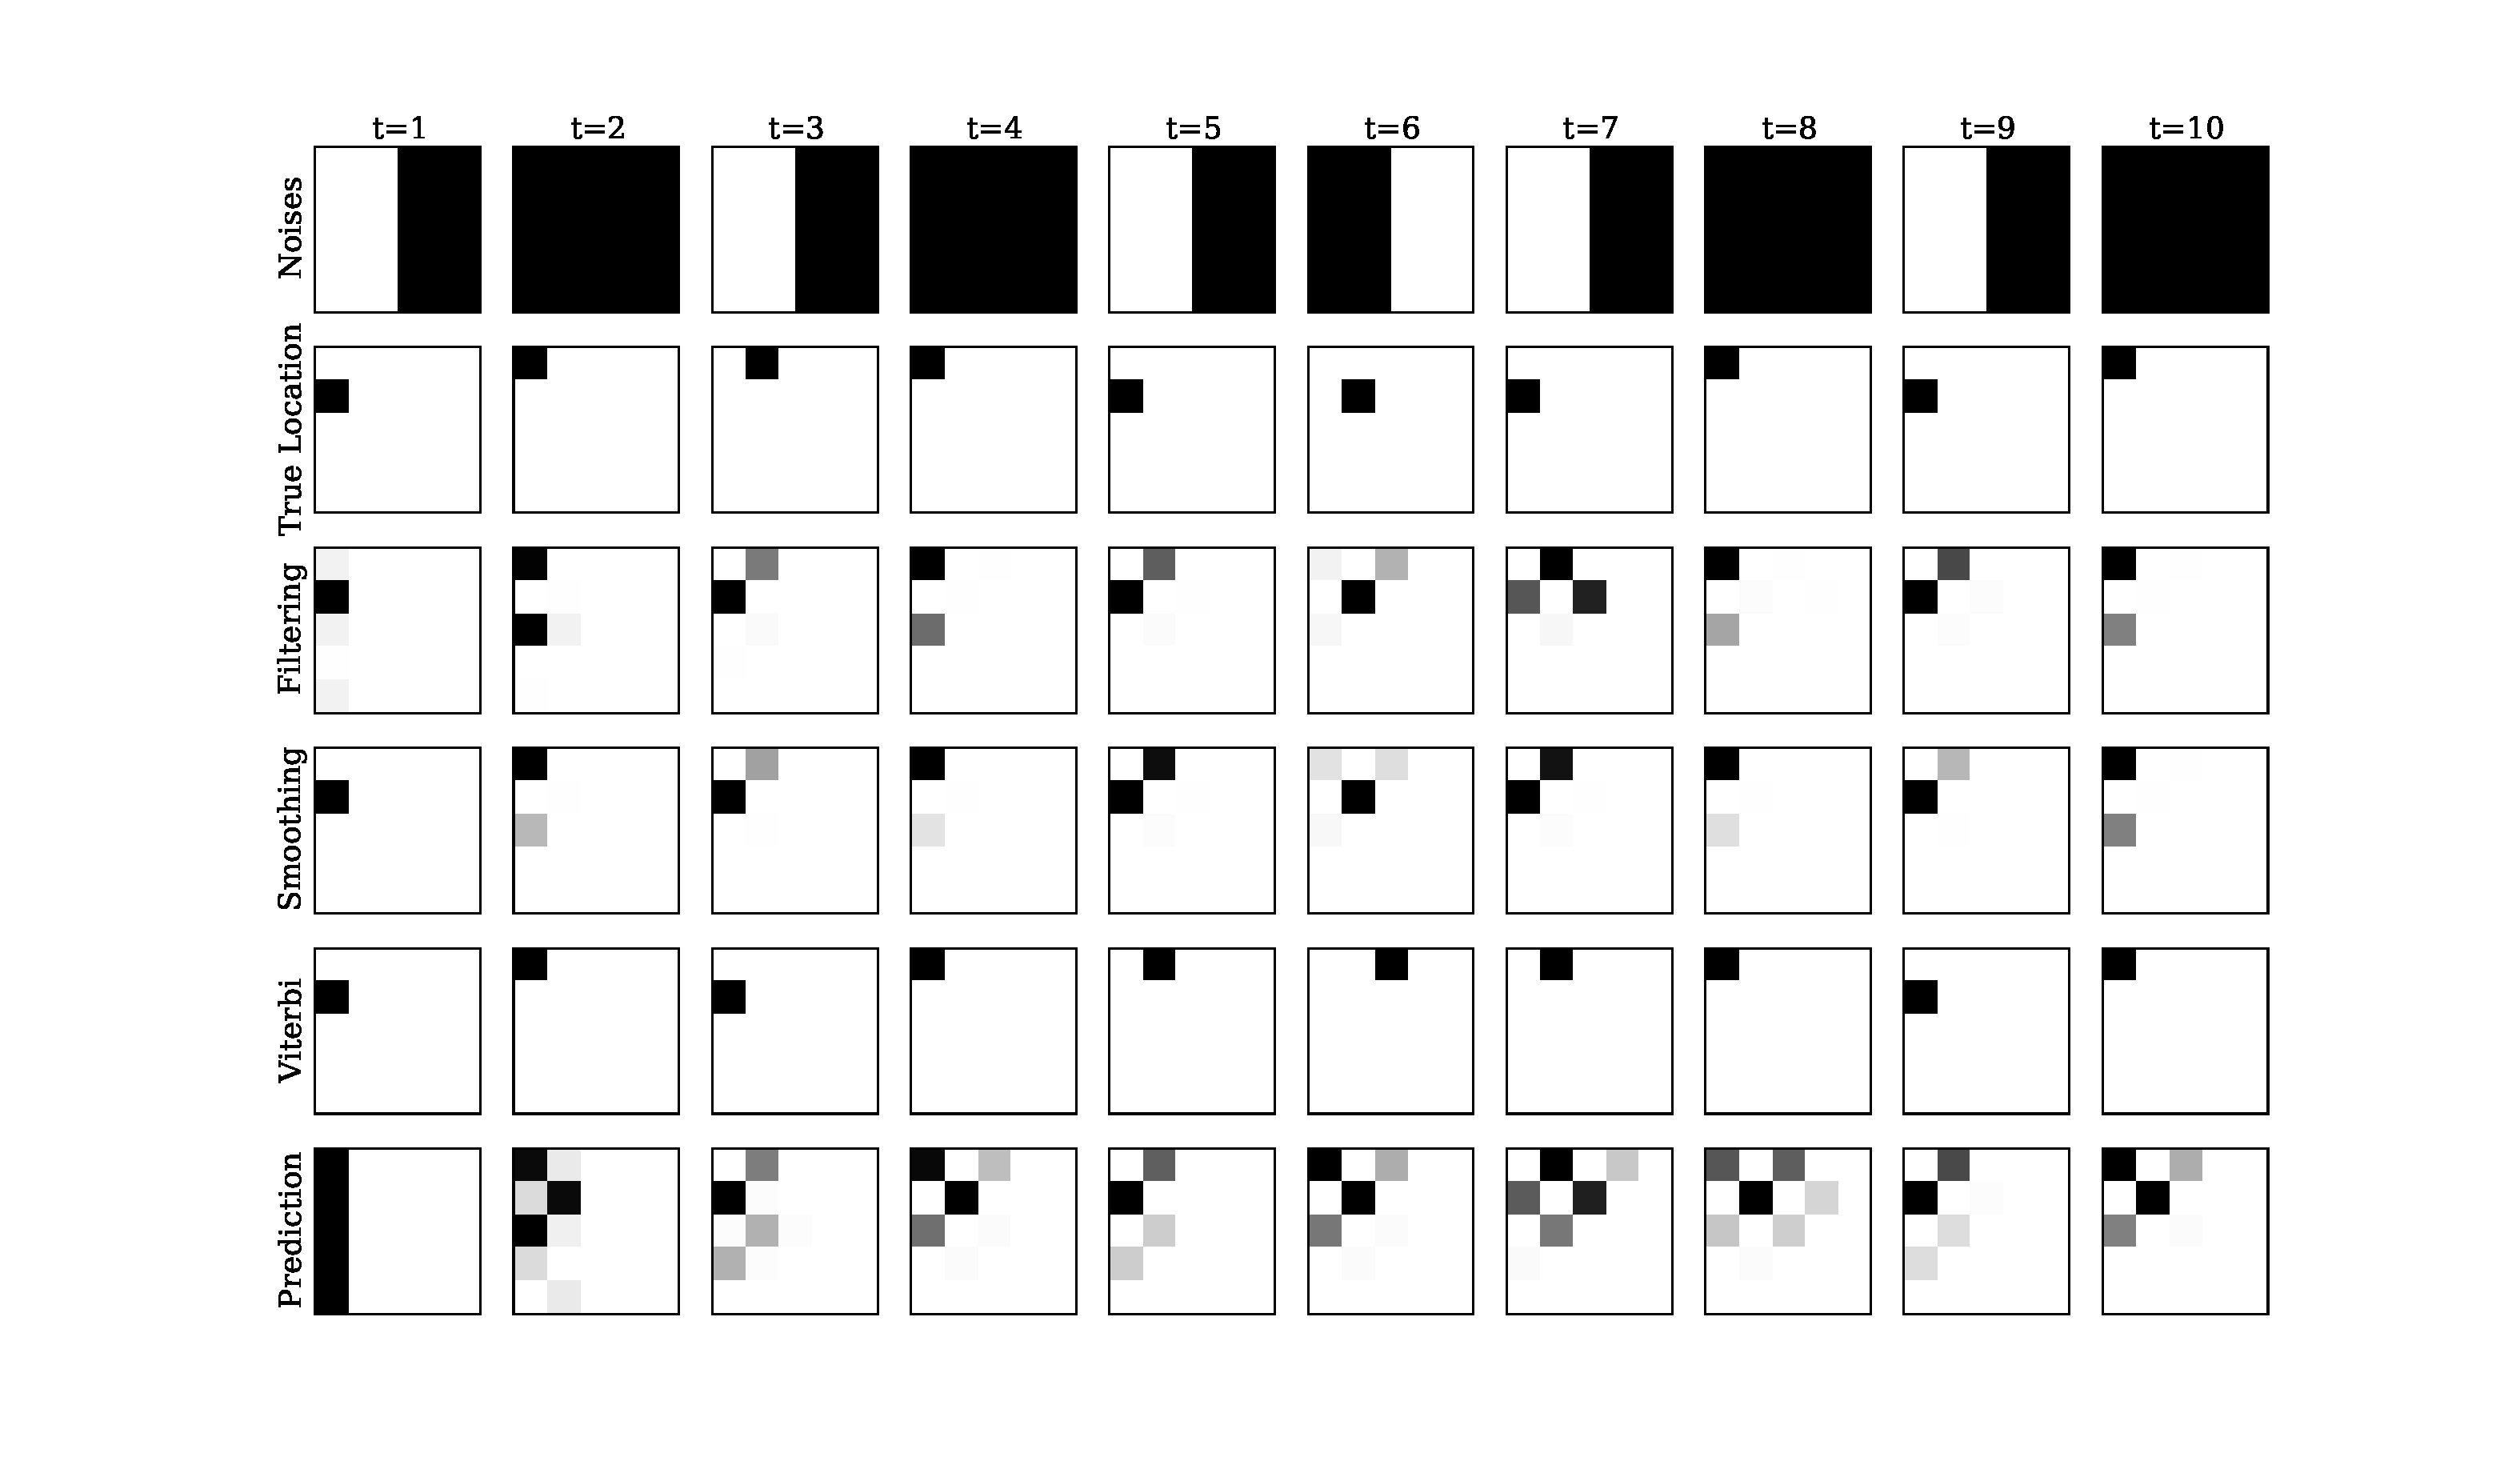
\includegraphics[scale=0.30]{burglar_inference.pdf}
\caption{Burglar Problem: Filter, Smoothing and Viterbi Decoding}
\label{fig_burglar_inference}
\end{figure}

\begin{figure}[H] 
\centering
\includegraphics[scale=0.30]{burglar_prediction.pdf}
\caption{Burglar Problem: Prediction}
\label{fig_burlgar_prediction}
\end{figure}


\subsection{Continuous Models}
In the previous

\bibliographystyle{plain}
\bibliography{research}

\end{document}